%#BIBTEX bibtex Si3N4
\documentclass[twocolumn,amsmath,amssymb,a4paper,prb,superscriptaddress,floatfix]{revtex4-1}
\usepackage[dvipdfmx]{graphicx}
\usepackage{natbib}
\usepackage{multirow}
\usepackage{amsmath}
\usepackage{bm}
\usepackage{mathrsfs}
\usepackage{url}
\usepackage{color}
\usepackage{ulem}
\begin{document}

\title{First-principles calculation of the lattice thermal
conductivities of $\alpha$-, $\beta$-, and $\gamma$-Si$_3$N$_4$}

\author{Kazuyoshi Tatsumi} \email{k-tatsumi@imass.nagoya-u.ac.jp}
\affiliation{aAdvanced Measurement Technology Center, Institute of
Materials and Systems for Sustainability, Nagoya University, Chikusa,
Nagoya 464-8603, Japan}
\affiliation{Center for Elements Strategy
Initiative for Structural Materials, Kyoto University, Sakyo, Kyoto
606-8501, Japan}

\author{Atsushi Togo}
\affiliation{Center for Elements Strategy Initiative for Structural
Materials, Kyoto University, Sakyo, Kyoto 606-8501, Japan}

\author{Isao Tanaka}
\affiliation{Center for Elements Strategy Initiative for Structural
Materials, Kyoto University, Sakyo, Kyoto 606-8501, Japan}
\affiliation{Department of Materials Science and
Engineering, Kyoto University, Sakyo, Kyoto 606-8501, Japan}
\affiliation{Nanostructures Research Laboratory, Japan Fine Ceramics
Center, Atsuta, Nagoya 456-8587, Japan}

\begin{abstract}
Lattice thermal conductivities of $\alpha$-, $\beta$- and
$\gamma$-Si$_3$N$_4$ single crystals are investigated from {\it
ab-initio} anharmonic lattice dynamics, within the single-mode
relaxation-time approximation of the linearized phonon Boltzmann
transport equation. At 300 K, the lattice thermal conductivity of
$\alpha$-Si$_3$N$_4$ is calculated as $\kappa_{xx}=69$ and
$\kappa_{zz}=99$ (in units of Wm$^{-1}$K$^{-1}$). For
$\beta$-Si$_3$N$_4$, $\kappa_{xx}=73$ and $\kappa_{zz}=198$ are
obtained, that is consistent with the reported experimental values of 69
and 180, respectively. The difference of anisotropy between
$\alpha$-Si$_3$N$_4$ and $\beta$-Si$_3$N$_4$ is originated from their
characteristic difference in the phonon band structures, although their
crystal structures are similar in their local atomic coordinates. In
$\alpha$-Si$_3$N$_4$, acoustic-mode phonons below 6 THz are the main
heat carriers. In $\beta$-Si$_3$N$_4$, the phonon modes up to 12 THz
contribute to the lattice thermal conductivity.
%
In $\gamma$-Si$_3$N$_4$, $\kappa=81$ is obtained. The distribution of
phonon mode contributions to lattice thermal conductivity along phonon
frequency is found to closely resemble $\kappa_{xx}$ of
$\beta$-Si$_3$N$_4$ although the phonon lifetimes of
$\gamma$-Si$_3$N$_4$ are twice shorter than those of $\beta$-Si$_3$N$_4$.
\end{abstract}

\maketitle

\section{Introduction}
Several nitride insulators showing good thermal conductivities are
important for heat sink materials used at elevated
temperatures. Wurtzite-type w-AlN, which has an Adamantine
(diamond-like) crystal structure, was noted by Slack et al.~\cite{slack} as
exhibiting a large thermal conductivity of over 100 WK$^{-1}$m$^{-1}$.
Si$_3$N$_4$ has been more recently recognized as one of the good
thermally conductive insulators. Remarkable advances in technologies
related to the densification of the ceramic body and microstructural
control have pushed the thermal conductivities of Si$_3$N$_4$ ceramics
up to 177 WK$^{-1}$m$^{-1}$.~\cite{zhou,hirao,watari,hirosaki} Since Si$_3$N$_4$ ceramics also exhibit
high mechanical strength at elevated temperatures, they are regarded as
ideal for use in various applications, such as engine components, gas
turbines, and heat sink substrates of power semiconductor devices.

\textcolor{red}{At atmospheric pressure}, Si$_3$N$_4$ exists in one of
two phases, $\alpha$ and $\beta$, both in the hexagonal lattice system,
which are generally considered to be low- and high-temperature phases,
respectively.~\cite{zhou,hirosaki,riley} Their crystal structures are commonly formed by
%
\textcolor{red}{stacking of basal layers}
%
of SiN$^4$ tetrahedra.
%
\textcolor{red}{The stacking manners in $\alpha$ and
$\beta$-Si$_3$N$_4$ are as ABAB.. and ABCDABCD.., respectively, where
the CD layers are mirror images of AB with respect to the plane.~\cite{hampshire}}
%
The unit cell periodicity of the $\alpha$ phase is approximately two
times longer than that of the $\beta$ phase, with lattice constants of c
= 5.62~\cite{yashima} and 2.91~\cite{boulay} \AA, respectively. In addition to the $\alpha$ and
$\beta$ phases,
%
\textcolor{red}{the cubic spinel $\gamma$-Si$_3$N$_4$ can be obtained
	upon compression and simultaneous-in-situ heating.~\cite{zerr,zhang} The reported
transition pressures were scattered from 10 to 36 GPa depending on the
experimental conditions. The produced $\gamma$ phase can be
experimentally quenched to atmospheric pressure and room temperature.}

By using high-resolution thermoreflectance microscopy, Li {\it et al.}~\cite{li}
reported the thermal conductivities of individual rod-shaped
$\beta$-Si$_3$N$_4$ grains in a ceramic to be 69 and 180
Wm$^{-1}$K$^{-1}$ along the $a$ and $c$ axes, respectively, and thus
revealed the large anisotropy in thermal conductivity. Takahashi {\it
et al.}~\cite{takahashi} recently developed a technique whereby $\beta$-Si$_3$N$_4$
grains are coated with graphene of relatively high magnetic
susceptibility, enabling them to align their c axes along the external
magnetic field. Based on this large anisotropy in thermal
conductivity, it was proposed that the textural structure of rod-shaped
$\beta$-Si$_3$N$_4$ grains would increase their thermal conductivity to
a level matching or exceeding that of w-AlN.

Although the fabrication of millimeter-sized $\beta$-Si$_3$N$_4$ single
crystals has been reported~\cite{yamamoto}, the thermal conductivity of no isolated
single crystal of any Si$_3$N$_4$ phase has yet been experimentally
determined. It was proposed~\cite{watari-trans} that the anisotropy in the thermal
conductivity of $\beta$-Si$_3$N$_4$ phase grains may not stem from the
intrinsic crystal properties, but rather, from the selective removal of
crystal defects along the c axis of the grains. Theoretically,
Hirosaki {\it et al.}~\cite{hirosaki-md} estimated the room-temperature lattice thermal
conductivities (LTCs) $\kappa$$_{xx}$ and $\kappa$$_{zz}$ of
$\alpha$-Si$_3$N$_4$ to be 105 and 225, and $\kappa$$_{xx}$ and
$\kappa$$_{zz}$ of $\beta$-Si$_3$N$_4$ to be 170 and 450, respectively,
by applying the Green-Kubo formulation to the molecular dynamics method
with the interatomic potentials proposed by Vashishta {\it et al.} The
ratio of the LTCs along the a and c axes agreed well with the
experimental results obtained by Li {\it et al.}; however, the absolute
values were more than two times larger than the experimental results.
%
\textcolor{red}{The LTC of the $\gamma$ phase was estimated only by the
Slack model.~\cite{morelli}}
%
While the thermal conductivity of polycrystalline $\beta$-Si$_3$N$_4$
has been significantly improved~\cite{zhou,hirao,watari,hirosaki}, our basic knowledge of, for example,
the thermal conductivity tensors of the different crystal phases remains 
insufficient.
   
\textcolor{red}{A decade ago, {\it ab-initio} calculations based on
Boltzmann transport theory combined with the harmonic and anharmonic
interatomic force constants by density functional theory were presented
by Broido {\it et al.}.~\cite{broido} Because of the computational costs, the
calculated materials were limited for several crystals having a few
atoms in the unit-cell. Semi-empirical approaches with {\it ab-initio}
harmonic phonon states were adopted to understand underlying mechanisms
of phonon transport of relatively large systems, whose thermal
conductivity was supposed to be experimentally clarified.~\cite{thomas} Thanks to
the increasing computational power, the larger systems containing more
than 20 atoms per unit-cell have been investigated~\cite{mukhopadhyay} by the full {\it
ab-initio} calculations within the single-mode relaxation time
approximation (RTA).~\cite{ward-ltc,esfarjani-ltc} This approach gives systematic estimations
for LTCs of the large systems whose intrinsic LTCs are not
experimentally established and the full solution of Boltzmann transport
equation is still difficult to be calculated due to the computational
cost. The Si$_3$N$_4$ polymorphs, which contain 14 or 28 atoms per
primitive cell, are the case.}

\textcolor{red}{The {\it ab-initio} LTC approach has many crystalline
systems whose underlying mechanisms of the phonon thermal transport are
still not clarified. The {\it ab-initio} LTC calculation can now be
applied to the other larger systems. The previous study of the LTC in
many polymorphs of the zincblende and wurtzite structures showed that
the difference in the stacking orders of the atom planes between these
structures affects little their LTC values.~\cite{phono3py} On the other hand, the
previous experimental~\cite{hirosaki,hirai} and theoretical~\cite{hirosaki-md,morelli} studies of thermal
conductivities of $\alpha$- and $\beta$-Si$_3$N$_4$ suggest that this is
not true for $\alpha$- and $\beta$-Si$_3$N$_4$.  
While the point group symmetry determines the anisotropy of
LTC tensors, the degree of the anisotropy depends on the material, which can be examined by
the first principles LTC calculation as the case of Ge$_2$Sb$_2$Te$_5$
in ref.~\onlinecite{mukhopadhyay-ltc}. $\gamma$-Si$_3$N$_4$ can be regarded as an ideally simple
representative of the spinel-type structure, because it has a single
non-transition metal element for cations. By comparing the $\gamma$
phase with the $\alpha$/$\beta$ phases, we can shed light on the
underling mechanisms of the LTC of the spinel-type structure.}

\textcolor{red}{The present study aims to qualitatively understand the
LTC tensors among the three Si$_3$N$_4$ phases by means of the {\it
ab-initio} approach. After the methodology
section, we examine the validity of the present LTC results first. Then
the harmonic phonon states and phonon lifetimes
are examined to find what microscopic property determines the characteristics in the LTC.}

\section{Computational procedures}
\subsection{Lattice thermal conductivity calculation}
The LTCs were calculated by solving the linearized Boltzmann
transport equation (LBTE) within the single-mode RTA.
%
\textcolor{red}{We also tried the direct-solution of LBTE~\cite{chaput-direct} and shortly
leave its calculated LTC values in the following section. However the
difference of LTCs between by the single-mode RTA and by the direct
solution was found minor for our discussion. Therefore we limited our
research based on the single-mode RTA to take advantage of the intuitive
closed form of LTCs with the single-mode RTA.}

In the following sections, we denote a phonon mode by
$\lambda=(\mathbf{q},p)$ by the set of the phonon wave vector
$\mathbf{q}$ and band index $p$. the relaxation time due to
phonon-phonon scattering was obtained as reciprocal of linewidth,
$\tau_{\lambda,\text{ph-ph}}=(2\Gamma_\lambda)^{-1}$, where the
linewidth that we employed in this study is as follows:
\begin{align}
 \label{eq:linewidth}
 &\Gamma_\lambda = \frac{18\pi}{\hbar^2}
  \sum_{\lambda' \lambda''}
  \bigl|\Phi_{-\lambda\lambda'\lambda''}\bigl|^2 \times \nonumber \\ 
 &\left\{ (n_{\lambda'} + n_{\lambda''}+1) 
   \delta(\omega_\lambda-\omega_{\lambda'}-\omega_{\lambda''}) \right.
   + \nonumber \\ 
 &\;\;(n_{\lambda'}-n_{\lambda''})
  \left[\delta(\omega_\lambda +\omega_{\lambda'}-\omega_{\lambda''})
 \right. 
 \left. -\left. \delta(\omega_\lambda - \omega_{\lambda'}+\omega_{\lambda''})
 \right]\right\}.
\end{align}
Here $\omega_\lambda$ is the harmonic phonon frequency of the phonon
mode $\lambda$,
$n_\lambda=[\exp(\hbar\omega_\lambda/\mathrm{k_B}T)-1]^{-1}$ shows the
Bose-Einstein distribution, and $\Phi_{\lambda\lambda'\lambda''}$
denotes the three-phonon-scattering
strength. $\Phi_{\lambda\lambda'\lambda''}$ was obtained by usual
coordinate transformation of third-order force constants from direct
space to phonon space.~\cite{phono3py} The second- and third-order real-space force
constants were obtained from the {\it ab-initio} calculation, whose
details are written in the next section.

In order to compare the more realistic results of the calculated LTC
with the experimental data, the isotopic scattering effect due to the
natural isotope distribution was taken into account according to the
second-order perturbation theory.~\cite{tamura} With the relaxation times of the
phonon-phonon scattering and isotropic scattering,
$\tau_{\lambda,\text{ph-ph}}$ and $\tau_{\lambda,\text{iso}}$, the total
relaxation time for a phonon mode was assumed to be
$1/\tau_{\lambda} = 1/\tau_{\lambda,\text{ph-ph}} +
1/\tau_{\lambda,\text{iso}}$, according to Matthiessen's rule.

These LTCs were calculated with the phonon-phonon interaction
calculation code PHONO3PY~\cite{phono3py}, while the harmonic phonon states were
analyzed with the phonon calculation code
PHONOPY~\cite{phonopy}. These codes have been
developed and maintained by the authors in this study.

\textcolor{red}{The available experimental thermal conductivity data of
the Si$_3$N$_3$ system have been measured on the polycrystalline samples
and not measured from any single crystals. In order to consider the
effect of various lattice defects in the polycrystalline samples, such
as grain boundaries, impurities, and vacancies, we crudely took them
into account by a relaxation time
$\tau_{\lambda,\text{bs}}=L/|\mathbf{v}_\lambda|$ of a phonon boundary
scattering model, where $\mathbf{v}_\lambda =
\nabla_{\mathbf{q}}\omega_\lambda$ is the group velocity and $L$ a
parameter regarding to the boundary mean free path. We consider
$\tau_{\lambda,\text{bs}}$ as a variable parameter and included it to
LTCs according to Matthiessen's rule.}

The closed form of the LTC tensors within RTA were obtained via 
\begin{align}
 \label{eq:kappa}
 \boldsymbol{\kappa}(T) = \frac{1}{N_\mathbf{q}\Omega} \sum_\lambda
 \tau_\lambda(T) \mathbf{v}_\lambda \otimes \mathbf{v}_\lambda c_\lambda(T),
\end{align}
where $T$ is the temperature, $N_\mathbf{q}$ is the number of
$\mathbf{q}$-points, $\Omega$ is the unit cell volume, and $c_\lambda$
is the mode heat capacity. To analyze the LTC in detail, we calculate
the cumulative thermal conductivity:
\begin{align}
 \label{eq:cum-kappa}
 \boldsymbol{\kappa}^\text{c}(\omega) = \frac{1}{N_\mathbf{q}\Omega}
 \int_0^\omega \sum_\lambda
 \tau_\lambda(T) \mathbf{v}_\lambda \otimes \mathbf{v}_\lambda
 c_\lambda(T) \delta(\omega'-\omega)d\omega'.
\end{align}

\subsection{Computational details}
The IFCs were calculated using the first-principles projector augmented
wave method~\cite{paw} (VASP code~\cite{vasp-1996,vasp-1995, vasp-1999}). The generalized
gradient approximation (GGA) parameterized by Perdew, Burke, and
Ernzerhof~\cite{pbe} was used for the exchange correlation potential. A plane
wave energy cutoff of 500 eV was employed. The crystal structures were
optimized until the convergence in the residual forces acting on the
constituent atoms was less than $10^{-6}$ eV/\AA. The structural
optimization was firstly performed for a temperature of 0 K and 0
GPa. Here the temperature and pressure were considered only for the
electronic system and the zero point lattice vibration was not taken
into account. The calculated lattice parameters were $a=7.808$ \AA~ and
$c=5.659$ \AA~ for the $\alpha$ phase, $a=7.660$ \AA~ and $c=2.925$ \AA~%
for the $\beta$ phase, and $a=7.787$ \AA~ for the $\gamma$ phase, which
agree with the experimental data~\cite{yashima,boulay,paszkowicz-gSi3N4} within +0.7 \% errors. The
lattice volume optimized at 0 K and 0 GPa within the local density
approximation (LDA)~\cite{lda} for the exchange correlation potential was 143.8
\AA$^3$ for $\beta$-Si$_3$N$_4$, being 3 \% smaller than the volume with
GGA, which is a typical volume contraction of LDA. In our test using
$\beta$-Si$_3$N$_4$ at 0 K and 0 GPa showed that the LTC calculated with
LDA was larger by 2.6 \% than that with GGA. For our discussion, these
difference is enough small, therefore the impact of choice of exchange
correlation potential is considered to be minor in our study.

\begin{table}[ht]
 \caption{\label{table:LTC} Calculated lattice thermal conductivities
 (LTC) of $\alpha$-, $\beta$-, and $\gamma$-Si$_3$N$_4$
 (WK$^{-1}$m$^{-1}$) at 300 K with respect to several combinations of
 supercell sizes.}
 \begin{ruledtabular}
  \begin{tabular}{ccccc}
   \multirow{2}{*}{Phase}
   & \multicolumn{2}{c}{Supercell (\# of atoms)} &
   \multicolumn{2}{c}{LTC} \\
   \cline{2-5}
   & $3^\text{rd}$ FC & $2^\text{nd}$ FC & $xx$ & $zz$ \\
   \hline
   \multirow{6}{*}{$\alpha$}
   & $1\times 1\times 1$ (28) & $1\times
   1\times 1$ (28) & 37 &   57 \\ 
   & $1\times 1\times 2$ (56) & $1\times
   1\times 2$ (56) & 41 &   79 \\ 
   & $1\times 1\times 1$ (28) & $2\times
   2\times 2$ (224) & 56 &   81 \\ 
   & $1\times 1\times 2$ (56) & $2\times
   2\times 2$ (224) & 70 &   98 \\ 
   & $1\times 1\times 2$ (56) & $2\times
   2\times 3$ (336) & 69 &   97 \\ 
   & $1\times 1\times 2$ (56) & $3\times
   3\times 4$ (1008) & 69 &   99 \\ 
   \hline
   \multirow{5}{*}{$\beta$}
   & $1\times 1\times 2$ (28) & $1\times
   1\times 2$ (28) & 40 &   166 \\ 
   & $1\times 1\times 2$ (28) & $2\times
   2\times 4$ (224) & 75 &  208 \\ 
   & $1\times 1\times 3$ (42) & $2\times
   2\times 4$ (224) & 71 &  194 \\ 
   & $1\times 1\times 3$ (42) & $2\times
   2\times 5$ (280) & 72 &  197 \\ 
   & $1\times 1\times 3$ (42) & $3\times
   3\times 8$ (1008) & 73 &  198 \\ 
   \hline
   \multirow{3}{*}{$\gamma$}
   & $1\times 1\times 1$ (56) & $1\times
   1\times 1$ (56) & \multicolumn{2}{c}{75} \\ 
   & $1\times 1\times 1$ (56) & $2\times
   2\times 2$ (448) & \multicolumn{2}{c}{81} \\ 
   & $1\times 1\times 1$ (56) & $3\times
   3\times 3$ (56) & \multicolumn{2}{c}{82} \\ 
  \end{tabular}
 \end{ruledtabular}
\end{table}

Supercell and finite difference approaches were used to calculate the
IFCs.~\cite{wei-supercell} The $1\times 1\times2$, $1\times 1\times3$, and $1\times
1\times1$ supercells of the conventional unit cells were adopted for the
third-order IFCs of the $\alpha$, $\beta$, and $\gamma$ phases,
respectively, while the larger supercells $3\times 3\times4$, $3\times
3\times8$ and $2\times 2\times2$ were adopted for the respective
second-order IFCs. The constant atomic displacement distance was set to
0.03 \AA. Table \ref{table:LTC} shows the calculated LTC values for
several different choices of supercell sizes, indicating that our
calculated LTCs are reasonably converging with respect to the supercell
sizes.

Uniform $\mathbf{k}$-point sampling meshes of $4\times 4\times 2$,
$4\times 4\times 3$, and $3\times 3\times 3$ were used for the
third-order IFCs of the $\alpha$, $\beta$, and $\gamma$ phases. For the
former two phases the center of the $a^*$-$b^*$ plane were sampled
though the off-center grids along $c^*$-axis were sampled. For the
$\gamma$ phase, non-$\Gamma$ center mesh was used. For the second-order
IFC, the $\Gamma$-point was only sampled for the $\alpha$ and $\beta$
phase supercells and the only one $\mathbf{k}=(0.5, 0.5, 0.5)$ point was
sampled for the $\gamma$ phase supercell. The $\mathbf{q}$-point
sampling meshes of $14\times 14\times 16$, $14\times 14\times 32$, and
$22\times 22\times 22$ were used to calculate the LTCs in Eq.~(\ref{eq:kappa})
 for
the $\alpha$, $\beta$, and $\gamma$ phases.

To compare the calculated LTC with the experimental data measured at
finite temperatures, the experimentally measured lattice parameters may 
be preferred in case that they are known. We examined LTC of
$\beta$-Si$_3$N$_4$ at the equilibrium volumes ($V_\text{eq}(T)$) within the
quasi-harmonic approximation (QHA).~\cite{dove-p76} Except for this, the LTC values
were calculated with the equilibrium volume at 0 K ($V_\text{eq}(T=0)$).

We calculated volumetric thermal expansion coefficients and compared
them with the reported experimental values so as to check the validity
of the present calculation, because the thermal expansion is originated
from the anharmonicity of the interatomic potential as well as lattice
thermal conduction. The calculated values are 4.31 and 4.19 ($10^{-6}$
K$^{-1}$) at 300 K for the $\alpha$ and $\beta$ phases, while the
experimental values were 3.75 and 3.55 ($10^{-6}$ K$^{-1}$)~\cite{minikayev-alpha}. The present
calculation reproduced the experimental tendency where the $\alpha$
phase has a slightly larger thermal expansion coefficient than the
$\beta$ phase, supporting that the present calculations enable us to
qualitatively compare the LTC values of the Si$_3$N$_4$ phases.

In order to compare the microscopic phonon properties among the three
phases at the same conditions, those results calculated at 0 GPa are
shown and discussed. For the $\gamma$ phase, this means that we assume
the condition of virtually quenched $\gamma$ phase at 0 GPa from the
high pressure. To examine this, we calculated LTC of $\gamma$ phase at
10, 20, and 40 GPa as shown in Fig.~\ref{fig:S1}, where the
phenomenological behaviour of linear dependence of LTC with respect to
pressure with the calculated slope of 2.89 Wm$^{-1}$K$^{-1}$GPa$^{-1}$
was reproduced as similar to ref.~\onlinecite{andersson-pressure}. By this result, we consider that
the microscopic values are also varied smoothly with the pressure and
those at 0 GPa are meaningful to compare with the $\alpha$ and $\beta$
phases.

\subsection{Direct solution of LBTE}
The merit of the single-mode RTA is that we can intuitively understand
the qualitative character of LTC in terms of the relaxation time and
group velocity. The microscopic understanding of the full solution of
LBTE is still under the development~\cite{cepellotti-relaxons}
and the microscopic picture based
on collective phonons~\cite{hardy-collective}) will
require more complicate investigation although it is known that the
single-mode RTA solution of LBTE underestimates the full solution.~\cite{mukhopadhyay-ltc,ward-ltc}


For the $\beta$ phase, we partly adopted a direct solution of LBTE~\cite{chaput-direct},
which is one of the methods of LBTE full solutions. Because of the
larger computational demand for the direct solution, we calculated the
LTC with the $\mathbf{q}$-point sampling mesh of $10\times 10\times
26$. The LTC values of the direct solution without the isotope effect
were 74 and 237 WK$^{-1}$m$^{-1}$ for $\kappa_{xx}$ and $\kappa_{zz}$,
respectively, while the corresponding single-mode RTA values were 74 and
205 WK$^{-1}$m$^{-1}$. The $\kappa_{zz}$ of the direct solution was 16
\% larger than that of the single-mode RTA solution. Since the LTC
difference between the LBTE solutions is not significant and we expect
the physics on LTC is well understood within RTA in the current level of
our interest.

\section{Results and discussion}
\subsection{Lattice thermal conductivities}

\begin{table}[ht]
 \caption{\label{table:LTC-exp} Calculated thermal conductivities of
 $\alpha$-Si$_3$N$_4$ (trigonal), $\beta$-Si$_3$N$_4$ (trigonal),
 $\gamma$-Si$_3$N$_4$ (cubic), and wurtzite-type AlN (hexagonal) at 300
 K, compared with the experimental data. Theoretical bulk moduli $B$ in
 units of GPa, calculated by the authors by using the present band
 method, are presented in the fourth column.}
 \begin{ruledtabular}
  \begin{tabular}{cccccccccc}
   & \multicolumn{3}{c}{This work} & \multicolumn{3}{c}{\textcolor{red}{Ref. Theo.}}
   & \multicolumn{3}{c}{Ref. Expt.} \\
   \cline{2-10}
   & $\kappa_{xx}$ & $\kappa_{zz}$ & $B$ & $\kappa$ & $\kappa_{xx}$ & $\kappa_{zz}$ & $\kappa$ & $\kappa_{xx}$ & $\kappa_{zz}$ \\
   \hline
   $\alpha$-Si$_3$N$_4$ & 69 & 99 & 224 & 70\footnotemark[1] & 105\footnotemark[2] & 225\footnotemark[2] & 59\footnotemark[4] & - & -  \\
   $\beta$-Si$_3$N$_4$ & 73 & 198 & 237 & 250\footnotemark[1] & 170\footnotemark[2] & 450\footnotemark[2] & 122\footnotemark[5] & 69\footnotemark[6] & 180\footnotemark[6] \\
   $\gamma$-Si$_3$N$_4$ & 82 & - & 296 & 80\footnotemark[1] & - & - & - & - & - \\
   w-AlN & 218 & 190 & 196 & - & 240\footnotemark[3] & 212\footnotemark[3] & 285\footnotemark[7] & - & -
   \footnotetext[1]{Ref.~\onlinecite{morelli}, Slack model}
   \footnotetext[2]{Ref.~\onlinecite{hirosaki-md}, molecular dynamics (Green-Kubo)}
   \footnotetext[3]{Ref.~\onlinecite{phono3py}, LBTE full solution.}
   \footnotetext[4]{Ref.~\onlinecite{hirai}, thin film.}
   \footnotetext[5]{Ref.~\onlinecite{hirosaki}, poly-crystals.}
   \footnotetext[6]{Ref.~\onlinecite{li}, single crystalline grains of poly-crystals.}
   \footnotetext[7]{Ref.~\onlinecite{slack-aln}, single-crystal.}
  \end{tabular}
 \end{ruledtabular}
\end{table}

\textcolor{red}{ In Table \ref{table:LTC-exp}, the theoretical LTCs at
	300 K are compared with the previously reported experimental~\cite{hirosaki,hirai,li,slack-aln} and
	theoretical~\cite{morelli,hirosaki-md,phono3py} values. The present calculation results better agree
with the experimental $\kappa$$_{xx}$ and $\kappa$$_{zz}$ of
$\beta$-Si$_3$N$_4$, compared with the references of the Slack model~\cite{morelli}
and MD~\cite{hirosaki-md} results. The directional averages of the present $\kappa_{ii}$
in the $\alpha$, $\beta$, and $\gamma$ phases are 79, 115, and 81
Wm$^{-1}$K$^{-1}$. The value of the $\gamma$ phase is just as small as
that of the $\alpha$ phase, although the former phase shows the largest
bulk modulus ($B$) in Table \ref{table:LTC-exp}. It is generally known
that simple models through Debye temperature can provide only their
rough estimations. In section IV-C, we will investigate the detailed
mechanisms of the microscopic phonon properties behind the relative LTC
values.}

It can be seen that the theoretical LTCs of $\beta$-Si$_3$N$_4$ are
markedly more anisotropic than those of the $\alpha$ phase. The
theoretical LTCs of $\beta$-Si$_3$N$_4$ are in good agreement with the
corresponding experimental data for individual grains reported by Li
{\it et al.}~\cite{li}, indicates that the experimentally reported large
anisotropy in the thermal conductivities of $\beta$-Si$_3$N$_4$ stems
from the intrinsic properties of the crystal, rather than specific
defects induced during the sample preparation process. Among the
nitrides studied, the theoretical LTC of $\beta$-Si$_3$N$_4$ along the c
axis (194 WK$^{-1}$m$^{-1}$) is the closest to the values for
high-thermal-conductivity AlN.

\begin{figure}[ht]
 \begin{center}
  \includegraphics[width=0.90\linewidth]{Fig1.eps} \caption{(color
  online) \textcolor{red}{Temperature dependence of LTC for $\alpha$-
  and $\beta$-Si$_3$N$_4$. The LTC calculated with the fixed volume
  optimized at 0 K are shown by the solid curves. For
  $\beta$-Si$_3$N$_4$, the LTC with the boundary scattering effect are
  shown by broken curves. The LTC calculated with the equilibrium
  volumes at the temperatures are shown by crosses. Theoretical LTC for
  the bulk $\beta$-Si$_3$N$_4$ sample are also shown to be compared with
  the experimental LTC (filled circles) of the bulk sample.}
  \label{fig:Fig1_338} }
 \end{center}
\end{figure}

Fig.~\ref{fig:Fig1_338} shows the theoretical LTCs of the $\alpha$ and
$\beta$ phases as a function of $T$, in comparison with the reference
experimental data,
%
\textcolor{red}{which were measured from the polycrystalline
samples. The data of the polycrystalline bulk samples cannot be directly
compared with the theoretical LTC tensors because the microstructures of
the bulk samples affect the thermal conductivities. We calculate
theoretical LTC values of the polycrystalline bulk sample as $\kappa = w
\kappa_{xx} + (1-w) \kappa_{zz}$, with an adjustable parameter $w$
between 0 and 1 for the least square differences from the experimental
data.}

The temperature dependence of the theoretical LTC, induced by
$\tau_{\lambda\text{ph-ph}}$, is close to $T^{-1}$ because 300 K is high
enough to approximate the linewidth in Eq.~(\ref{eq:linewidth}) by a
high-temperature limit for these phases.
%
\textcolor{red}{In Fig.~\ref{fig:Fig1_338}-a, the temperature dependence
of the experimental data of a chemically vapor-deposited
$\alpha$-Si$_3$N$_4$ sample~\cite{hirai} is deviated from $T^{-1}$ considerably,
intersecting the theoretical curves of the $\kappa$$_{xx}$ and
$\kappa$$_{zz}$ at 400 and 600 K, respectively. Thus no value of $w$
adjusts the theoretical LTC to the experimental curve. Assuming the
underestimation of SMRTA $\sim$15 \% from the results of the $\beta$
phase, the full solution of LBTE would cure the disagreement only
partly. Including the simple phonon lifetime of boundary scattering,
$\tau_{\lambda,\text{BS}} =L/v_\lambda$, into the total phonon lifetime
according to Matthiessen's rule, could not explain the discrepancy as
well. $\tau_{\lambda,\text{BS}} =L/v_\lambda$ with $L = 0.75$
$\mu\text{m}$, which was much smaller than the experimental grain size
10 $\mu\text{m}$, decreases the room-temperature theoretical $\kappa$$_{xx}$ and
$\kappa$$_{zz}$ values toward the experimental value, but severely
underestimated the experimental values at the high temperature side. At
present, the reason for the discrepancy between the theoretical and
experimental behaviors is unclear. Although the crystal structure of the
experimental sample was characterized as $\alpha$-Si$_3$N$_4$,
significant lattice defects might exist in the as-deposited sample as
pointed out by Hirosaki {\it et al.}~\cite{hirosaki-md}, and many of them might be
diminished in the high temperature side of the measurement.}

The experimental values of the $\beta$-phase ceramic bulk~\cite{hirosaki} fall well
between the calculated values of $\kappa$$_{xx}$ and $\kappa$$_{zz}$.
%
\textcolor{red}{The experimental data are nearly parallel to the
theoretical $\kappa$$_{xx}$ and $\kappa$$_{zz}$ curves.}
%
If we compare the experimental values with $\sum_i \kappa_{ii}/3$, which is
a simple directional average, the calculation shows slight
underestimations with respect to the experiment, which can be understood
from an experimentally tailored microstructure containing large
$\beta$-Si$_3$N$_4$ grains selectively grown along the c axis.~\cite{hirosaki}

\textcolor{red}{The theoretical curve adjusted with $w=0.37$ explains
well the experimental data of the poly-crystal bulk in
Fig.~\ref{fig:Fig1_338}-b. For the effects of lattice defects most of
which are grain boundaries, we included $\tau_{\lambda,\text{BS}}$ with
$L = 1$ $\mu\text{m}$ to further fit the theoretical curve ($w=0.44$) to
the experimental data. The $L$ value is similar to the average grain
size (2 $\mu\text{m}$) of the experimental polycrystalline
sample~\cite{hirosaki}. Fig.~\ref{fig:Fig1_338}-b also contains the experimental
$\kappa$$_{xx}$ and $\kappa$$_{zz}$ at room temperature by filled
squares, which are in-between the theoretical components with and
without $\tau_{\lambda,\text{BS}}$.}

\textcolor{red}{The LTC values with the equilibrium lattice volumes
($V_\text{eq}$) at 300, 600, 900, 1200 and 1500 K within QHA are plotted
by crosses in Fig.~\ref{fig:Fig1_338}. The deviations due to the thermal
expansions were less than 1 \%. Therefore this effect is negligible for
the present study. The degree of the differences is similar to the case
of Si and Ge~\cite{ward-ltc}.}

\subsection{v$_\lambda$ on reciprocal plane}


Fig.~\ref{fig:Fig2_ver2_338} shows the $\kappa^\text{c}(\omega)$ of the
$\beta$ phase along two inequivalent directions and their ratios as an
indicator of the anisotropic thermal conductivities; isotope effects are
not considered in this figure. We can clearly see that the phonon modes
in the frequency range of 0--12 THz contribute significantly to
LTC. Interestingly, in the same frequency range, the anisotropy of
$\kappa^\text{c}(\omega)$ increases monotonically. Thus, we can focus on
this frequency range when we investigate the anisotropy of the thermal
conductivity of the $\beta$ phase in detail.

\begin{figure}[ht]
 \begin{center}
  \includegraphics[width=0.90\linewidth]{Fig2.eps}
  \caption{Theoretical cumulative sums of mode LTC
  $\boldsymbol{\kappa^\text{c}(\omega)}$ (see Eq.~(\ref{eq:cum-kappa})) of
  $\beta$-Si$_3$N$_4$ along the $a$ and $c$ axes, i.e.,
  $\kappa^\text{c}_{xx}(\omega)$ and $\kappa^\text{c}_{zz}(\omega)$,
  respectively, and their ratios,
  $\kappa^\text{c}_{zz}(\omega)/\kappa^\text{c}_{zz}(\omega)$.
  \label{fig:Fig2_ver2_338} }
 \end{center}
\end{figure}

\begin{figure*}[ht]
 \begin{center}
  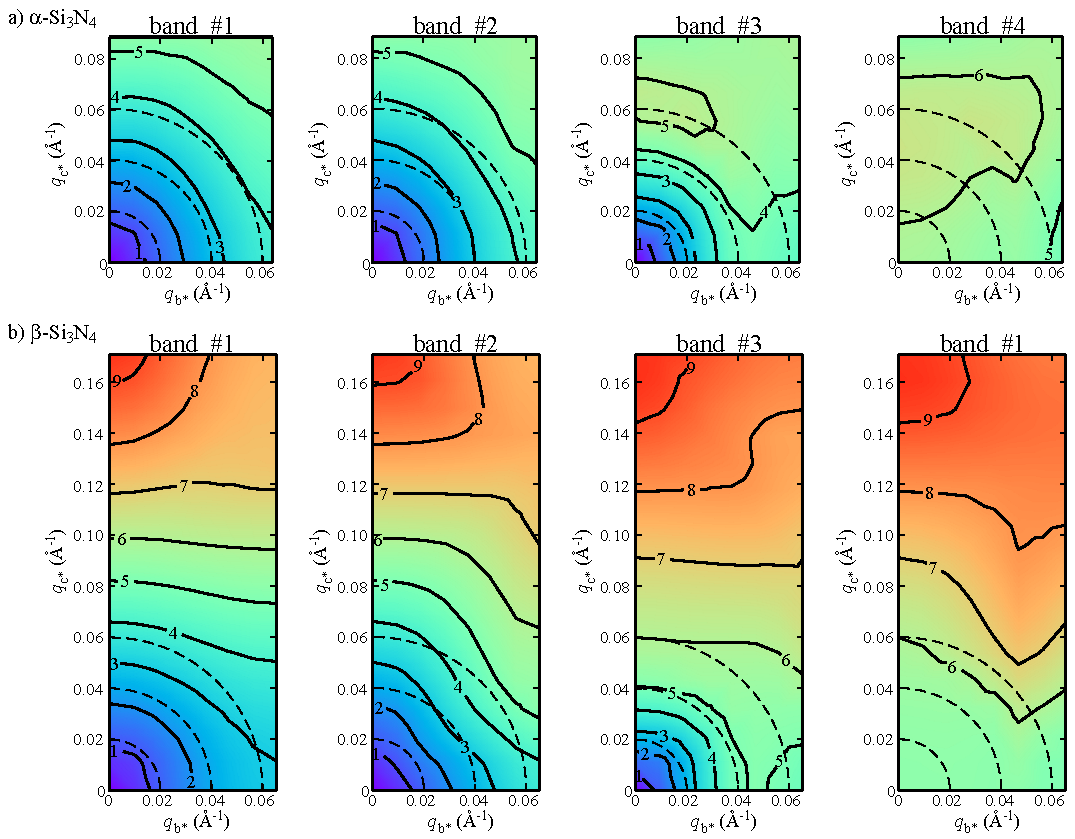
\includegraphics[width=0.90\linewidth]{Fig3_338_resize2_times.eps} \caption{(color
  online) Contour maps of phonon frequency (THz) on the $b^*$-$c^*$
  planes of Brillouin zones. The maps for the four lowest-frequency
  phonon states are shown. The frequency landscapes are formed by simply
  connecting the frequencies of the same band indices, assigned by
  ascending order of frequency at the respective q
  points. \label{fig:Fig3_338} }
 \end{center}
\end{figure*}

The cross-sections of the phonon frequency distributions on the
$b^*$-$c^*$ planes in the first Brillouin zones are shown in
Fig.~\ref{fig:Fig3_338}. The cross-sections of other planes containing
the $c^*$ axis did not differ much from Fig.~\ref{fig:Fig3_338}; thus,
we focus on the results for the $b^*$-$c^*$ planes as representative of
all such planes. We show only the frequencies of four modes from the
lowest frequency because they contribute significantly to LTC. In
Fig.~\ref{fig:Fig3_338}-b of the $\beta$ phase, the iso-frequency lines
in $0.06 \le q_{c^*} \le 0.12$ (\AA$^{-1}$) are almost parallel to the
$q_{b^*}$ axis, i.e., the group velocities in this section are nearly
along the $c$ axis. The cross-sections in Fig.~\ref{fig:Fig3_338}-b
indicate that the four modes of the $\beta$ phase, in a significantly
large part of the phonon states in the Brillouin zone, have group
velocities oriented along the $c$ axis, resulting in a much larger LTC
along the $c$ axis than along the $a$ ($b$) axis in this
phase. Fig.~\ref{fig:Fig3_338}-a shows that the frequency distributions
and group velocities of $\alpha$-Si$_3$N$_4$ are fairly isotropic.

\subsection{v$_\lambda$ on Brilloin Zone paths}


\textcolor{red}{Figure \ref{fig:Fig4_ver5_338} shows the phonon band diagrams 
of the three Si$_3$N$_4$ phases.
The entire band diagrams are almost identical to those reported earlier~\cite{kuwabara,xu}.
However, here we focus on the group velocities on high-symmetry paths for the 
entire frequency range. This has not been investigated by the previous works. 
}

\begin{figure}[ht]
 \begin{center}
  \includegraphics[width=0.90\linewidth]{Fig4_ver5_338_resize2_woDOS.eps}
  \caption{(color online) 1st Brillouin Zones (left) and calculated phonon band diagrams (right) for three Si$_3$N$_4$ phases.
  \label{fig:Fig4_ver5_338} }
 \end{center}
\end{figure}

In the band diagram of $\beta$ (Fig.~\ref{fig:Fig4_ver5_338}-b), along
the $\Gamma$--A path, the acoustic phonon branches highlighted in red
increase their frequencies almost linearly from the $\Gamma$-point to
the zone boundary of the A-point around 10 THz. Their gradients are
large, so the group velocity components along the c axis maintain high
values. Normally, optical branches are flat; however, the upper branches
along the same path, highlighted in blue, also have significantly large
group velocity components along the c axis.

In contrast, the corresponding acoustic branches in the $\alpha$ phase
highlighted in red in Fig.~\ref{fig:Fig4_ver5_338}-a do not increase
their frequencies as much as those of the $\beta$ phase. This is because
the $\Gamma$--A path length of the $\alpha$ phase is approximately half
that of $\beta$. The lattice constant c of $\alpha$ is nearly twice that
of $\beta$, owing to the difference in the stacking manner of the basal
layers. The frequency maxima along the $\Gamma$--A path are around 7 THz,
rather close to the maxima along the $\Gamma$--K and $\Gamma$--M paths
(around 5 THz). Moreover, the upper branches highlighted in blue are
relatively flat, like the upper branches along the $\Gamma$--K and
$\Gamma$--M paths.

%The total DOS of the $\alpha$ phase shows a distinct peak at ~6 THz, as
%indicated by an arrow, where the phonon branches become dispersionless
%over the entire path in the band diagram. The first peaks of $\alpha$
%and $\beta$ are related to the L-points or the Brillouin zone (BZ) edges
%with $c^* = 0.5$. The difference in their frequencies stems from
%difference in length between their BZs along $c^*$.

In Fig.~\ref{fig:Fig4_ver5_338}-c for the $\gamma$ phase, the acoustic phonon branches
highlighted in red show significant linear dispersion along the
L-$\Gamma$-X path. The frequencies of the longitudinal acoustic modes
are 14 and 12.5 THz at the L- and X-points. The frequencies of the
transverse acoustic modes are approximately half the values of the
longitudinal modes at the L-point and a factor of $1/\sqrt{2}$ smaller
than the longitudinal modes at the X-point, as in the case of fcc rare
gas solids~\cite{dove-p30}. The roughly constant gradients of the branches are large,
reflecting the large elastic constants of the $\gamma$ phase
\textcolor{red}{as shown in Table \ref{table:LTC-exp}.} 
%

\subsection{Distributions of phonon lifetimes and their impact on the
  LTCs of the three phases}

\begin{figure}[ht]
 \begin{center}
  \includegraphics[width=0.90\linewidth]{Fig5_338_rev.eps}
  \caption{(color online) Frequency-distributions of phonon lifetimes
  (a), DOS, (b) and cumulative thermal conductivities (c) among the
  three Si$_3$N$_4$ phases. \label{fig:Fig5_338_rev} }
 \end{center}
\end{figure}

The distributions of the phonon lifetimes are shown in
Fig.~\ref{fig:Fig5_338_rev}-a. The DOS and cumulative thermal
conductivities are attached in Fig.~\ref{fig:Fig5_338_rev}-b and c, to
allow the distributions of the phonon states and their contributions to
LTC to be examined with ease. The common trend is that the phonon
lifetime decreases with increasing $\omega$in the lower frequency
region ($<6$ THz). Most of the phonon lifetimes of the $\alpha$ phase
are larger than those of the $\beta$ phase in this frequency
region. However, above 6 THz, the phonon lifetimes of the three phases
are distributed similarly and roughly constant. The values for $\gamma$
are as low as half those for $\alpha$ and $\beta$.
%
\textcolor{red}{The vertical lines in Fig.~\ref{fig:Fig5_338_rev} show
the maximum frequencies of the Debye model, $\nu_\text{D}$. We use
$\nu_\text{D}$ as a roughly estimated frequency-boundary between the
acoustic and optical phonon modes. From Fig.~\ref{fig:Fig5_338_rev} and
the band diagrams of Fig.~\ref{fig:Fig4_ver5_338}, we can highlight the
frequency-dependent microscopic mechanisms on 1) the large $\kappa_{zz}$
of the $\beta$ phase, and 2) the relatively small LTC value of the
$\gamma$ phase.}

\textcolor{red}{Only the $zz$ component of
$\boldsymbol{\kappa}^\text{c}(\omega)$ for the $\beta$ phase increases
much as  increases beyond $\nu_\text{D}$. It is a characteristic point
of the $\beta$ phase that the phonon modes of $\omega > \nu_\text{D}$
largely contribute to the $\kappa_{zz}$. They contribute approximately
1/3 of the total $\kappa_{zz}$. Because the phonon lifetimes in this
frequency range are not large, a large number of phonon modes with large
z components of group velocities, including optical phonon modes like
the upper branches highlighted by blue in Fig.~\ref{fig:Fig4_ver5_338},
contribute to the $\kappa_{zz}$. In contrast to the $\beta$ phase, the
$zz$ component of the $\alpha$ phase does not increase much above
$\nu_\text{D}$, as all the phonon branches reach to the Brillouine zone
boundary and decreased their group velocities.}

\textcolor{red}{The $\gamma$ phase has the largest $\nu_\text{D}$, and
the smallest phonon lifetimes above 6 THz. Thus the
frequency-distributions of the acoustic phonon states and their
lifetimes of the $\gamma$ phase are least compatible for high LTC among
the three phases, while the optical phonon modes do not have large group
velocities. This is the reason for the relatively small LTC of the
$\gamma$ phase in spite of the large group velocities of the acoustic
branches.}

\begin{figure}[ht]
 \begin{center}
  \includegraphics[width=0.80\linewidth]{Fig6_338_beta.eps}
  \caption{(color online) Hypothetical cumulative thermal conductivity
  for $\beta$-Si$_3$N$_4$. \label{fig:Fig6_338_beta} }
 \end{center}
\end{figure}

Our argument that the anisotropic group velocities are responsible for
the anisotropic LTC of the $\beta$ phase can be simply confirmed by
hypothetically setting the two ($C_\lambda$ and $\tau_\lambda$) of the
microscopic four terms ($C_\lambda$, $v_\lambda$, $\tau_\lambda$, and
DOS) constant. In Fig.~\ref{fig:Fig6_338_beta} are the corresponding
hypothetical cumulative thermal conductivities,
\begin{align}
 \boldsymbol{\kappa}^{\text{c}'}(\omega) =
 \frac{\mathrm{k_B}\tau}{N_q\Omega} \int^\omega_0 \sum_\lambda
 \mathbf{v}_\lambda
 \otimes \mathbf{v}_\lambda \delta(\omega' - \omega_\lambda)d\omega'
\end{align}
The mode heat capacity was set to Boltzmann’s constant, $\mathrm{k_B}$,
as the high-temperature approximation, which is a reasonable
approximation for $\omega < 19$ THz, and we set $\tau$ to 20 ps and let
the of the $\beta$ phase approach at $\omega=12$ THz for simplicity.
%
\textcolor{red}{$\boldsymbol{\kappa}^{\text{c}'}(\omega)$ shows as large
anisotropy as $\boldsymbol{\kappa}^{\text{c}}(\omega)$, confirming that the anisotropy in LTC is caused by the
anisotropic group velocities while insensitive to the distribution of
phonon lifetimes.}

\begin{figure}[ht]
 \begin{center}
  \includegraphics[width=1.00\linewidth]{Fig7.eps} \caption{(color
  online) Comparison between derivatives of cumulative thermal
  conductivity and DOS weighted with squared group velocity. a)
  $\alpha$-Si$_3$N$_4$ and b) $\beta$-Si$_3$N$_4$.  \label{fig:Fig7} }
 \end{center}
\end{figure}

\textcolor{red}{Moreover, to clearly show the different degrees of the
anisotropy between $\alpha$- and $\beta$-Si$_3$N$_4$, in 
Fig.~\ref{fig:Fig7}, we compare
the derivative of the cumulative thermal conductivity,
d$\boldsymbol{\kappa}^\text{c}/d\omega$, with the DOS weighted with the
squared group velocity. The intensities of the latter is calculated by
\begin{align}
 v_{ii}^2(\omega) = \frac{1}{N_q\Omega}\sum_\lambda
 \mathbf{v}_{\lambda,i}^2 \delta(\omega - \omega_\lambda)
\end{align}
}

\textcolor{red}{For both of $\alpha$- and $\beta$- Si$_3$N$_4$, we can
see the similarity between the derivatives of $\kappa_{zz}$ and
$\kappa_{xx}$ with the DOS weighted with $v_{\lambda,z}^2$ and
$v_{\lambda,x}^2$. For the higher frequencies than approximately 15 THz,
the mode heat capacities decrease and suppress the intensities of the
derivatives. The areal intensity of the derivatives and the weighted DOS
are consistent for the lower frequency region. Therefore the difference
in the anisotropy of the LTC between the $\alpha$ and $\beta$ phases
reflects the difference in the group velocities, which is originated
from the difference in the stacking order of the basal planes.}

\section*{ACKNOWLEDGMENTS}
The present work was partly supported by Grants-in-Aid for Scientific
Research of MEXT, Japan (Grant No. 15K14108 and ESISM (Elements Strategy
Initiative for Structural Materials) of Kyoto University).

\appendix
\section{Pressure dependence of LTC of $\gamma$-phase}
\begin{figure}[ht]
 \begin{center}
  \includegraphics[width=0.80\linewidth]{S1.eps} \caption{(color online)
  Pressure dependence of LTC of $\gamma$-Si$_3$N$_4$.  \label{fig:S1} }
 \end{center}
\end{figure}


\bibliography{Si3N4}
\end{document}
